\chapter{Conclusões Finais}
% \begin{figure}[H]
%         \center
%         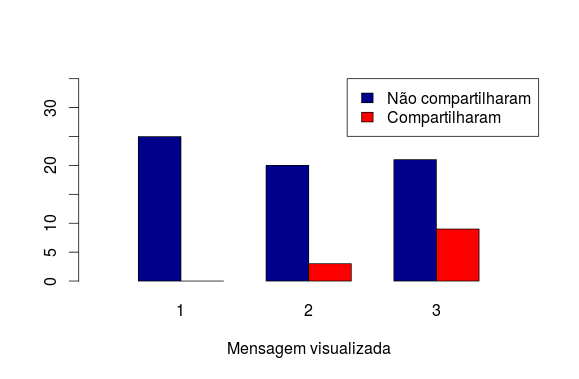
\includegraphics[scale=.7]{./figuras/barchart-compartilhamentos.png}
%         \caption{Oi}
%         \label{fig:barchart}
%     \end{figure}
% \begin{itemize}
%     \item Resumir, em um parágrafo, tudo o que eu fiz e descobri.
% \end{itemize}

% \section{Contribuições}
% \begin{itemize}
% \item Quando e como as pessoas compartilham?
% \item Por que as pessoas compartilham em grupos do Facebook e não compartilham no Stack Overflow/Quora, etc.? 
% \item Compartilhar pergunta do Stack Overflow fez diferença no meu experimento?
% \item Alguma estratégia testada funcionou? Quem funcionou mais? Quem funcionou menos?
% \item Uma análise do comportamento dos usuários de sites q\&a em relação ao compartilhamento;
% \item Uma análise sobre a influência do compartilhamento de perguntas na obtenção, ou não, de respostas em sites q\&a;
% \item Uma análise sobre a interferência de certos cenários na tentativa de promover o compartilhamento de perguntas em sites de q\&a e as influências dos compartilhamentos nos cenários na obtençãom, ou não, de respostas.
% \end{itemize}

\section{Limitações e Trabalhos Futuros}
falar que eu até tentei ver algo sobre a utilidade de se compartilhar uma pergunta nas redes sociais, mas não deu pra concluir nada pq só tinha dados de bots e as análises feitas deram resultados estranhos (mostrar os resultados) que precisam ser esmiuçados em mais detalhes para refletir sobre o real significado disto;

testar novas mensagens,

utilizar uma quantidade maior de perguntas e atrair uma quantidade maior de usuários;

atrair usuários de outros sites diferentes do stack overflow em português;

Qual é a ligação entre tais resultados e o que existe na literatura?

preciso de mais dados para saber se compartilhar pode representar uma boa estratégia para atrair mais respostas, mas tou achando que não de acordo com a análise feita com os dados reais...
% \begin{itemize}
% \item Escopo reduzido das duas pesquisas qualitativas e da pesquisa quantitativa;
% \item Como trabalho futuro sugere-se expandir este escopo e ver se usuários do Stack Overflow em inglês (o mais popular de todos) se comportariam diferente;
% \item Ver se o mesmo experimento quantitativo feito para o Stack Overflow em inglês traria resultados diferentes (compartilhar pergunta do Stack Overflow em inglês faria diferença? o que eu acho disto? por que eu penso assim?);
% \item Abordar outros sites da plataforma Stack Exchange e ver se os resultados seriam os mesmos (acredito que não - explicar o motivo pelo qual eu acredito que os resultados seriam diferentes neste caso).
% \end{itemize}